% ==============================================
% 電気・情報関係学会北陸支部連合大会
% 講演論文投稿用 pLaTeX2e 版テンプレートファイル(2段組)
% Usage: platex jhes2022_platex_utf8_template.tex
% ==============================================

\documentclass[a4paper,10pt]{jarticle}

\usepackage{here} % 図挿入位置のパッケージ
\usepackage[dvipdfmx]{graphicx}

% ==============================================
% page format
%  textwidth  = paperwidth(210mm) -oddsidemargin(13mm) -evensidemargin(13mm)
%  textheight = paperheight(297mm) -topmargin(20mm-header分) -bottommargin(18mm)
% ==============================================
  \setlength{\paperwidth}{210mm}
  \setlength{\textwidth}{\paperwidth}
  \addtolength{\textwidth}{-13mm} % oddside margin
  \addtolength{\textwidth}{-13mm} % evenside margin
  \setlength{\oddsidemargin}{-1in}
  \addtolength{\oddsidemargin}{13mm} % ここで左右を調節

  \setlength{\paperheight}{297mm}
  \setlength{\textheight}{\paperheight}
  \addtolength{\textheight}{-28mm} % 文章領域の高さの調整
  \setlength{\topmargin}{-15mm}    % ここで上下位置を調節

  \setlength{\headheight}{0in}
  \setlength{\headsep}{0in}
  \setlength{\columnsep}{10mm}

\makeatletter
\renewcommand{\section}{\@startsection{section}{1}{\z@}
  {1.5\Cvs \@plus.5\Cvs \@minus.2\Cvs}
  {.5\Cvs \@plus.3\Cvs}%
  {\reset@font\large\bfseries}}   % section見出しの文字サイズをlargeに変更
\renewcommand{\subsection}{\@startsection{subsection}{2}{\z@}
  {1.5\Cvs \@plus.5\Cvs \@minus.2\Cvs}
  {.5\Cvs \@plus.3\Cvs}
  {\reset@font\normalsize\bfseries}} % subsectoin見出しの文字サイズをnormalsizeに変更
\makeatother

  \pagestyle{empty}

\begin{document}
\twocolumn[

\begin{center}
{\Large 2023 年度電気・情報関係学会北陸支部連合大会}\\
\vspace{-2mm}\rule{\textwidth}{1mm}
\end{center}
% ==============================================
% 原稿はここから
% ==============================================

% 講演題目 =====================================
\hspace*{33mm} 
\begin{minipage}{118mm}  % 210mm-13mm-13mm-33mm-33mm
\begin{center}    % 左づめの場合はflushleft
{\Large \bf
マルチモーダル入力を用いた\\電力使用量の異常値予測のための最適な特徴量選択
\\ \vspace*{4mm}	% 複数行の場合,強制改行して,行間を調整

}
\end{center}
\end{minipage}

\vspace*{4mm}	% 行間を調整

%%%%%%%%%%%%%%%%%%%%%%%%%%%%%%%%%%%%%%%%%%%%%%%%%%%%%%%%%%%%
% 著者名(所属) =====================================
\hspace*{33.0mm} % 講演番号用空欄
\begin{minipage}{118mm}  % 210mm-13mm-13mm-33mm-33mm
\begin{center}    % 左づめの場合はflushleft
{\large
{山名田 恭吾(福井大学大学院工学研究科)}\\{黒岩 丈介} {小高 知宏(福井大学大学院工学研究科)}\\{白井 治彦(福井大学工学部)}
}
\end{center}
\end{minipage}

\vspace*{6mm}	% ここで行間を調整
]

%%%%%%%%%%%%%%%%%%%%%%%%%%%%%%%%%%%%%%%%%%%%%%%%%%%%%
% 本文 =====================================
%%%%%%%%%%%%%%%%%%%%%%%%%%%%%%%%%%%%%%%%%%%%%%%%%%%%%%%%%%%%%%%%
\section{はじめに}
\vspace{-2mm}
%%%%%%%%%%%%%%%%%%%%%%%%%%%%%%%%%%%%%%%%%%%%%%%%%%%%%%%%%%%%%%%%%%
近年,原子力発電の稼働が減り,原子力発電よりも発電コストの高い火力発電の稼働量が増えている.
電力使用量予測を行うことによって,
長期的には化石燃料の適切な調達,短期的には電力使用量の増減に合わせて発電所の稼働状態を
調節することができる.
つまり,電力使用量の予測を行なうことは重要である\cite{kamata}.
このような考えのもと,
我々は,マルチモーダル入力を用いた深層学習手法による電力使用量予測に関する研究を行なってきた.
先行研究では,電力使用量の時系列ごとのデータの予測については高い予測精度を示していたが,電力使用量が突然跳ね上がる異常値の予測精度は高くなかった.
安定した電力供給を行うためには,このような異常使用が発生することを予測できることが重要となる.
そこで,本研究では,機械学習による異常値の予測を行うための適切な特徴量を明らかにすることを目的としている.
%%%%%%%%%%%%%%%%%%%%%%%%%%%%%%%%%%%%%%%%%%%%%%%%%%%%%%%%%%
%\vspace{-7mm}
%\section{LightGBM}
%\vspace{-2mm}
%
%本実験では,LightGBM という従来の勾配ブースティング決定木の学習プロセスを高速化した機械学習手法を用いて予測を行う.
%このモデルは 2017 年に Microsoft が開発した教師あり学習のデータ分析方法の一つである.
%LightGBM は,データインスタンスが小さな勾配の時,そのデータインスタンスを除外して学習を高速化する Gradient-based One-Side Sampling(GOSS)と,排他的な特徴量を束ねることで特徴量の数を減らす Exclusive Feature Bundling(EFB)の 2 つを用いることで効率的な学習を行うモデルである[2].
%決定木を深さ方向ではなく,葉の方向に分割することで計算量を削減することができる.

% https://www.mdpi.com/2075-4418/11/9/1714
% https://ieeexplore.ieee.org/stamp/stamp.jsp?arnumber=9284642
%%%%%%%%%%%%%%%%%%%%%%%%%%%%%%%%%%%%%%%%%%%%%%%%%%%
%\begin{figure}[b!]
%  \vspace{-3mm}
%  \includegraphics[width=.95\linewidth]{fig/LightGBM.eps}
%  \vspace{-3mm}
%  \caption{LightGBM における葉の成長}
%  \label{fig:leaf}
%\end{figure}
%%%%%%%%%%%%%%%%%%%%%%%%%%%%%%%%%%%%%%%%%%%%%%%%%%%%%%%%%%%%%%%%%%
\vspace{-7mm}
\section{LightGBM を用いた電力使用量予測}
%%%%%%%%%%%%%%%%%%%%%%%%%%%%%%%%%%%%%%%%%%%%%%%%%%%%%%%%%%%%%%%
\vspace{-2mm}
\subsection{実験手法}
\vspace{-2mm}
%%%%%%%%%%%%%%%%%%%%%%%%%%%%%%%%%%%%%%%%%%%%%%%%%%%%%%%%%%%%%%%%%%%%%%%%
本実験では,電力使用量は東京電力パワーグリッド株式会社が提供している東京電力の 2016 年 4 月から 2022 年 3 月までの電力使用量のデータを用いた.
電力使用量及びその微分値以外に,電力使用量との相関が強い,気温・天気・降水量・異常値・時間・曜日・移動平均を全て適切に加工し,特徴量とした.
データは,8:2 で学習データとテストデータに分割した.
入力に対して 1 時間後の電力使用量を予測し,予測結果の異常値予測精度を算出する.
また,予測値と実測値を最小値 0,最大値 1 に規格化した後,RMSE(平均平方二乗誤差)を用いてトレンド予測精度についても評価する.

予測実験には,LightGBM を用いた\cite{rufo}.
LightGBM は,
従来の勾配ブースティング決定木の学習プロセスを高速化した機械学習手法である.
このモデルは 2017 年に Microsoft が開発した教師あり学習のデータ分析方法の一つである.
LightGBM は,データインスタンスが小さな勾配の時,そのデータインスタンスを除外して学習を高速化する Gradient-based One-Side Sampling(GOSS)と,排他的な特徴量を束ねることで特徴量の数を減らす Exclusive Feature Bundling(EFB)の 2 つを用いることで効率的な学習を行うモデルである.
%決定木を深さ方向ではなく,葉の方向に分割することで計算量を削減することができる.
%%%%%%%%%%%%%%%%%%%%%%%%%%%%%%%%%%%%%%%%%
\vspace{-7mm}
\subsection{実験結果}
\vspace{-2mm}
%%%%%%%%%%%%%%%%%%%%%%%%%%%%%%%
\begin{table}[t!]
  \centering
  \caption{各特徴量を外したときの精度}
  \scalebox{.9}{
    \begin{tabular}{|l||c|c|c|}  \hline
      特徴量           &    寄与度(\%) &    精度(\%) &    下降度(\%)  \\ \hline \hline

      気温             &    22.6         &    93.4       &    -2.0         \\ \hline
      降水量           &    3.11         &    95.4       &     0.0         \\ \hline
      天気             &    2.10         &    95.4       &     0.0         \\ \hline
      異常値           &    3.61         &    88.2       &    -7.2         \\ \hline
      時間             &    21.3         &    83.6       &    -11.8         \\ \hline
      曜日             &    10.7         &    95.4       &     0.0         \\ \hline
      移動平均         &    21.0         &    83.6       &    -11.8         \\ \hline
      微分             &    15.8         &    94.7       &    -0.7         \\ \hline
    \end{tabular}
  }
  \vspace{-3mm}
  \label{tab:feature_rate_sa}
\end{table}
%%%%%%%%%%%%%%%%%%%%%%%%%%%%%%%%%%%%%%%%%%%%%
% \begin{figure}[b!]
%   \vspace{-3mm}
%   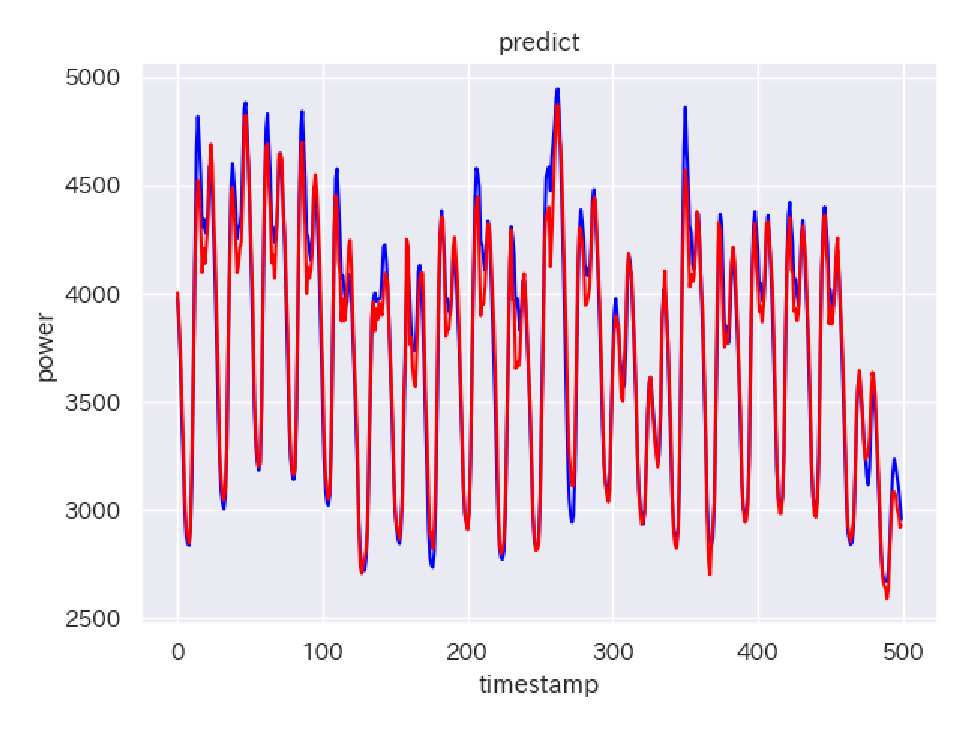
\includegraphics[width=.95\linewidth]{fig/light6_95.eps}
%   \vspace{-5mm}
%   \caption{電力使用量予測}
%   \label{fig:predict}
% \end{figure}
%%%%%%%%%%%%%%%%%%%%%%%%%%%%%%%%%%%%%%%%%%%%%%%%
予測実験結果を表 1 に与える.
異常値の予測精度が 95.4 \% ,RMSE(平均平方二乗誤差)が 0.0299 であった.
% また,表\ref{tab:feature_rate_sa}に各特徴量を外した時の異常値の予測結果を示す.
気温や時間,移動平均などは寄与度が高く,特徴量から外すと精度が大きく下がっている.
降水量や天気,曜日は寄与度が低いため,外しても精度はほとんど変化しなかった.
よって,これらの特徴量は異常値の予測に用いる必要がないことがわかる.
実際にこれら 3 つの特徴量を除外して予測した時の予測精度は 95.6 \% となったが,RMSE は 0.0350 となり,少し精度が下がっていた.
%%%%%%%%%%%%%%%%%%%%%%%%%%%%%%%%%
% \begin{table}[t!]
%   \centering
%   \caption{RMSE(0.0299からどれほど変化するか)}
%   \hspace{-2mm}
%   \scalebox{.9}{
%     \begin{tabular}{|l||c|}  \hline
%       特徴量           &    寄与度(\%)   \\ \hline \hline

%       気温             &    0.0432          \\ \hline
%       降水量           &    0.0308          \\ \hline
%       天気             &    0.0299          \\ \hline
%       異常値           &    0.0343          \\ \hline
%       時間             &    0.0778          \\ \hline
%       曜日             &    0.0354          \\ \hline
%       移動平均         &    0.0549          \\ \hline
%       微分             &    0.0318          \\ \hline
%     \end{tabular}
%   }
%   \label{tab:feature_RMSE}
% \end{table}
%%%%%%%%%%%%%%%%%%%%%%%%%%%%%%%%%%%%%%%%%%%%%%%%%%
\vspace{-7mm}
\section{考察}
\vspace{-2mm}
%%%%%%%%%%%%%%%%%%%%%%%%%%%%%%%%%%%%%%%%%%%%%%%%
LightGBM を用いて電力使用量の異常値予測を行った.
異常値の予測精度は寄与度の低い特徴量を除くことで 95.6 \% まで上げることができたが,
異常値区間を含めた全区間での RMSE が僅かに大きくなった.
%これは,多くの特徴量を用いることで電力使用量の振る舞いに,
%より適応した予測ができたためだと考えられる.
しかし,電力使用量予測では,電力使用量が急激に変化する異常値が発生することの予測が重要であり,
その他の区間の予測精度をある程度犠牲にしてでも異常値区間の予測精度を向上させる必要がある.
そのため,電力使用量予測では,特徴量は気温・異常値・時間・移動平均・電力使用量の微分を入力データとして使うことが適切であると考えられる.
%%%%%%%%%%%%%%%%%%%%%%%%%%%%%%%%%%%%%%%%%%%%%
\vspace{-6mm}
\begin{thebibliography}{9}
    \vspace{-2mm}
    % \bibitem[1]{}
    % Leon O. Chua,Valery I. Sbitnev,Sook Yoon,
    %   ``A Nonlinear Dynamics Perspective of Wolfram's New Kind of Science. Part2: Universal Neuron,''
    %   IJBC,Vol.13(9),pp.2379-2453,2003.
      
    \bibitem[1]{kamata}
    鎌田 真 , 市村 匠 , リカレント構造適応型 Deep Belief Network による時系列データの学習 , 計測自動制御学 会論文集 , Vol.54, No.8, 628/639(2018).
      
    \vspace{-2mm}

    \bibitem[2]{rufo}
    RUFO, Derara Duba, et al. Diagnosis of diabetes mellitus using gradient boosting machine (LightGBM). Diagnostics, 2021, 11.9: 1714.
    % https://www.mdpi.com/2075-4418/11/9/1714
\end{thebibliography}


\end{document}
